\documentclass[main.tex]{subfiles}
\begin{document}
\newpage
	\section{Introduction}
	This document describes how to install and run the different parts of our system. If you manually write the commands into your terminal you can leave out the \texttt{\textbackslash} in the commands, that go over two lines. They are only added so you can copy the commands into your terminal.\\
	In figure \ref{fig:architecture} you can see the architecture of our system.
	\begin{figure}[h]
\centering
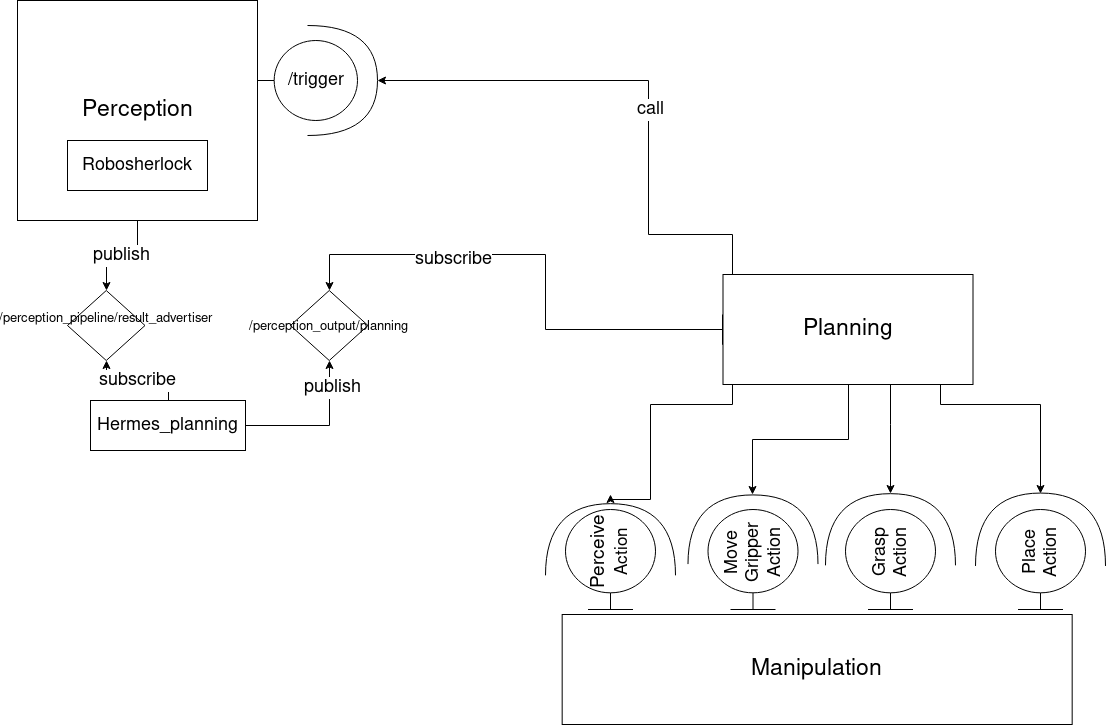
\includegraphics[width=0.8\textwidth]{architecture/architecture}
\caption{Architecture}
\label{fig:architecture}
\end{figure}
	
	\subsection{Prerequisites}
	
	For our system you will need \textbf{Ubuntu 16.04}.\\
	Furthermore Ros-Kinetic is needed. Instructions on how to install Ros can be found \href{http://wiki.ros.org/kinetic/Installation/Ubuntu}{here}. It is recommended to install the Desktop-Full version.\\
	You also have to setup your PC for the use of the HSR.
	A description on how to do that can be found \href{https://docs.hsr.io/manual_en/howto/pc_install.html}{here}\\
	The catkin\_tools package also needs to be installed. You find the instructions on how to install it \href{https://catkin-tools.readthedocs.io/en/latest/installing.html}{here}.\\
	To follow this guide you will also need python-wstool.
	You can install it by running this command:
	\begin{lstlisting}
sudo apt-get install python-rosinstall python-wstool
\end{lstlisting}
	
	\subsection{Workspaces}
	\subsubsection{Create a Workspace}
	The first step is to open the directory where you want to create the workspace.\\
	Now run the following commands.
	\begin{lstlisting}
source /opt/ros/kinetic/setup.bash
mkdir -p YOURWORKSPACENAME/src
cd YOURWORKSPACENAME/
catkin build 
\end{lstlisting}
	
	To load the environment of a workspace, you can run the command:
	\begin{lstlisting}
source devel/setup.bash
\end{lstlisting}
	in your workspace.
	
	\subsubsection{How we manage our Workspaces}
	
	We use three workspaces for our system, since using just one causes some problems.\\
	The first workspace contains the \nameref{sec:Manipulation} part (without Navigation).\\
	In the second workspace we installed the \nameref{sec:Planning} part.\\
	Everything else can be installed in the third workspace.\\
	\\
	Before starting a part of our system we run 
	\begin{lstlisting}
source devel/setup.bash
\end{lstlisting}
to source the relevant workspace in our Terminal.
	

\end{document}
